\chapter{Theoretical Framework}


\section{Standard Model of Fundamental Interactions}

This chapter present a brief description of the Standard Model of Fundamental Interactions (SM), indicating their origins, particle content, interactions and  lagrangians of different sectors.\\
\indent
The electroweak theory of the SM was proposed by Glashow, Weinberg and Salam \cite{Glashow:1961tr, Salam, PhysRevLett.19.1264} to describe the electromagnetic and weak interactions of quarks and leptons, which is based on the local gauge group  $SU(2)_{L}\otimes U(1)_{Y}$.
Combined with quantum chromodynamics (QCD), which is the theory of strong interactions between quarks and gluons, with local gauge group $SU(3)_{C}$, the model foresees a unified framework to detail these three forces of nature.\\
\indent
It is necessary to make a differentiation between different types of fundamental particles involved in the SM. The particles are divided into: bosons (particles of integer spin), responsible for transmitting the fundamental forces of the nature, and fermions (particles of half-integer spin) that are the constituents of matter. Since not all fermions have the same properties, they have been divided into two types: leptons and quarks. One of the differences is that quarks have fractional electric charge while the charge of the leptons are multiples of the electron charge. The quarks exhibit a very peculiar property called "confinement", which means that free quarks have not been observed. Quarks feel all interactions, but leptons are not affected by the strong force.\\
\indent
In particle physics, a generation is a division of elementary particles. Between generations, particles differ only in their mass. All interactions and quantum numbers are identical. There are three generations according to SM of particle physics. Each member of an higher generation has bigger mass than the corresponding particle of the previous generation. This hierarchy of mass causes particles to decay from high to low generations, which explains why ordinary matter (atoms) is made of particles of the first generation. Every atom is then composed of first generation particles. The second and third generations of charged particles do not form normal matter and are only seen in extremely high-energy environments. The table below  summarizes the main properties of fermions:

\begin{table}[h]
\footnotesize
\begin{center}
\begin{tabular}{|c|c|c|c|}\hline\hline
\multicolumn{4}{|c|}{\bfseries Fermions}\\ \hline\hline
  \textbf{Generation} & \ \textbf{Fermions} &  \textbf{Mass [MeV]}  &  \textbf{Charge} ($Q/\left|e\right|$) \\ \hline
  &u & $2.3$ & $2/3$   \\ \cline{2-4}
  & d & $4.8$ & $-1/3$ \\\cline{2-4} 
\raisebox{1.5ex}[0pt]{$1^{a}$}   &e & $0.511$ & $-1$   \\ \cline{2-4}
  & $\nu_{e}$ & $ < 2 \times 10^{-6}$ & $0$  \\ \hline
 &c & $1.275\times 10^{3}$ & $2/3$ \\ \cline{2-4} 
  &s & $95$ & $-1/3$ \\ \cline{2-4}
\raisebox{1.5ex}[0pt]{$2^{a}$} &$\mu$ & $105.66$ & $-1$ \\ \cline{2-4}
  & $\nu_{\mu}$ & $<  0.19$ & $0$ \\ \hline
&t & $173.21\times 10^{3}$ & $2/3$ \\ \cline{2-4}  
  &b & $4.18\times 10^{3}$ & $-1/3$ \\ \cline{2-4}
\raisebox{1.5ex}[0pt]{$3^{a}$} &$\tau$ & $1777$ & $-1$ \\ \cline{2-4}
 & $\nu_{\tau}$ & $< 18.2$ & $0$  \\ \hline\hline
\end{tabular}
\caption{Fermions Generations}\label{tab3} 
\end{center}
\end{table}

Unlike leptons, quarks are confined within hadrons, and they are not seen as physical particles. The masses of the quarks can not be measured directly, but can be determined indirectly through their influence on hadronic properties.\\
\indent
The different interactions are described in the quantum language in terms of bosons exchange between the constituents fermions.

\begin{table}[h]
%\centering
\resizebox{0.85\textwidth}{!}{\begin{minipage}{\textwidth}
\renewcommand{\arraystretch}{1.3}
\begin{tabular}{|c|c|c|c|c|}
\hline
\multicolumn{5}{|c|}{\textbf{Types of Interactions}}   \\ 
\hline
 Interaction & Gauge Group & Boson & Symbol & Relative Magnitude \\ 
\hline
Strong  & $SU(3)$ & gluons (8 types)  & $g$  & 1   \\ 
\hline
Electromagnetic  & $U(1)$  & photon  & $\gamma$  & $10^{-2}$  \\ 
\hline
Weak  & $SU(2)$  & intermediate vector bosons  & $W^{\pm}$, $Z^{0}$  & $10^{-7}$  \\ 
\hline
Gravitational  & ?  & Graviton (hypothetical)  & $G$  & $10^{-39}$  \\
\hline 
\end{tabular} 
\end{minipage}}
\caption{Fundamental Interactions \label{table:interactions} }
\end{table}

As the \cref{table:interactions} shows, there are four types of fundamental interactions.
The strong interactions are responsible to bind the quarks inside the proton and the neutron, while maintaining the neutron and the proton in the nucleus. The force between quarks is mediated by massless particles called gluons.
Electromagnetism is responsible for binding electrons in the atom, the atoms in the molecules, and intermolecular forces in liquids and solids. These interactions are mediated by the exchange of photons.
Weak interactions are typified by $\beta$ nuclear decay processes, which involves the emission of an electron and a neutrino by a radioactive nucleus.
The mediators of the weak force are bosons $W^{\pm}$ and $Z^{0}$, with masses of the order of
100 times the proton mass. Gravitational interactions act on all types of particles. 
As can seen from the \cref{table:interactions}, the relative magnitude of the gravitational interaction is very small, thus, for practical purposes it is not considered within the SM.

\begin{figure}[h]
  \centering
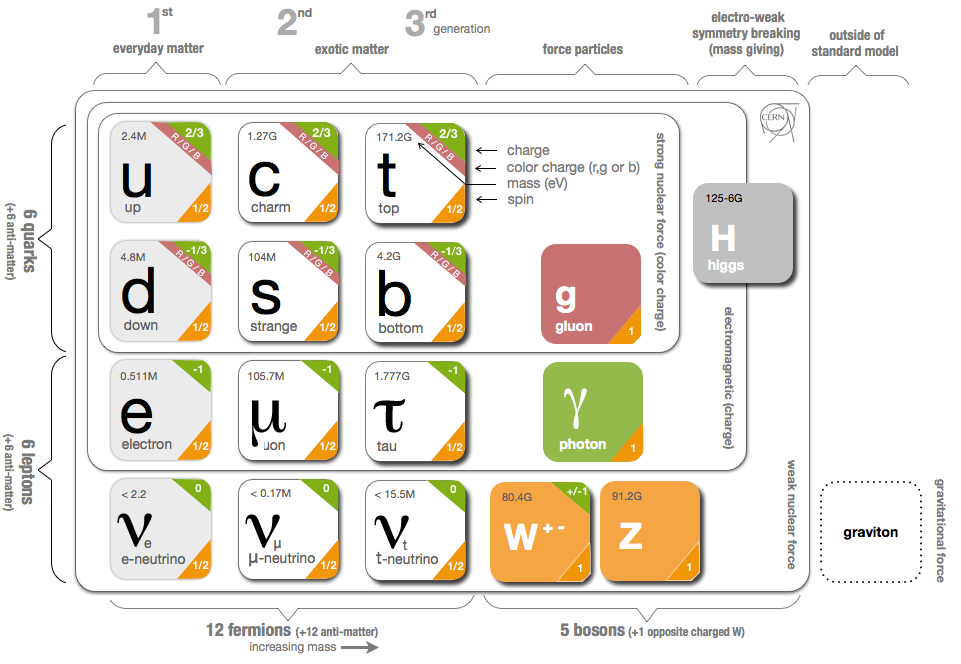
\includegraphics[width=12cm]{SM_chapter_plots/SM}
\label{SMfigure}\caption{Particles of the Standard Model}
\end{figure}

\subsection{Electroweak Interaction}

The SM propose a doublet representation for the left-handed fields and singlets for the right-handed fields:
\begin{eqnarray}
L^{i}=\left(
\begin{array}{c}
\displaystyle \nu_{e L}\\
\displaystyle e_{L}
\end{array}\right),
\left(
\begin{array}{c}
\displaystyle \nu_{\mu L}\\
\displaystyle \mu_{L}
\end{array}\right),
\left(
\begin{array}{c}
\displaystyle \nu_{\tau L}\\
\displaystyle \tau_{L}
\end{array}\right),
\qquad
Q^{i}=\left(
\begin{array}{c}
\displaystyle u_{L}\\
\displaystyle d_{L}
\end{array}\right),
\left(
\begin{array}{c}
\displaystyle c_{L}\\
\displaystyle s_{L}
\end{array}\right),
\left(
\begin{array}{c}
\displaystyle t_{L}\\
\displaystyle b_{L}
\end{array}\right).        
\end{eqnarray}
\begin{eqnarray}
e_{R}^{i} &=& \left\lbrace e_{R}, \mu_{R}, \tau_{R} \right\rbrace ,  \nonumber\\
u_{R}^{i} &=& \left\lbrace u_{R}, c_{R}, t_{R} \right\rbrace , \qquad d_{R}^{i} = \left\lbrace d_{R}, s_{R}, b_{R} \right\rbrace .
\end{eqnarray}
Where $i$ runs over the generations of fermions. The $L$ (left-handed) and $R$ (right-handed) indices appears because the projections operators were applied over the wave functions, where $\psi_{L}=P_{L}\psi$ and $\psi_{R}=P_{R}\psi$, with $P_{L}=(1-\gamma^{5})/2$ and $P_{R}=(1+\gamma^{5})/2$.\\
The free massless fermionic lagrangian is:
\begin{displaymath} 
\lagrangean_{f}=\frac{i}{2}\sum^{3}_{i=1}\left\{\:\bar{L}^{i}\:\not\! \partial\:L^{i}+\:  \bar{Q}^{i}\:\not\! \partial\:Q^{i}+\:\bar{e}_{R}^{i}\:\not\! \partial\:e_{R}^{i} + \:\bar{u}_{R}^{i}\:\not\! \partial\:u_{R}^{i} + \:\bar{d}_{R}^{i}\:\not\! \partial\:d_{R}^{i}  \right\}+\hbox{h.c}
\end{displaymath}
with $\bar{\psi}=\psi^{\dag}\:\gamma^{0}$.\\
The proposed Lagrangian must be invariant under local gauge transformations:
\begin{eqnarray}
\Psi_{i}\:'&=&\:\hbox{exp}\left[i\:\alpha(x)_{j}\sigma_{j}+i\:\beta(x)Y\right]\Psi_{i}\nonumber\\
\chi_{i}\:'&=&\:\hbox{exp}\left[i\:\beta(x)Y\right]\:\chi_{i}  
\end{eqnarray}
where $\Psi_{i}=\left\{L^{i},Q^{i}\right\}$ and $\chi_{i}=\left\{e_{R}^{i}, u_{R}^{i}, d_{R}^{i} \right\}$. Also, 
 $\alpha$ and $\beta$ are parameters belonging to the symmetry groups $SU(2)$ and $U(1)$ respectively, $\sigma_{j}$ are the Pauli matrices and $Y$ is the hypercharge.
In order to mantain the gauge invariance after the transformations, we have to introduce the covariant derivatives:
\begin{eqnarray}
D_{L}^{\:\mu}&=&\;\partial^{\mu}-\:i\:\left(g/2\right)\:\sigma_{j}\:A^{\mu}_{j}+\:ig'\:B^{\:\mu}\:Y\;\nonumber\\
D_{R}^{\:\mu}\:&=&\;\partial^{\mu}+\:i\:g'\:B^{\:\mu}\:Y\;\:
\end{eqnarray}
Finally we get:
\begin{eqnarray}\label{leptonico}
\lagrangean_{f}=\frac{i}{2}\sum^{3}_{i=1}\left\{\:\bar{L}^{i}\:\not\!\! D_{L}\:L^{i}+\:\bar{Q}^{i}\:\not\!\! D_{L}\:Q^{i}+\:  \bar{e}_{R}^{i}\:\not\!\! D_{R}\:e_{R}^{i}+\:  \bar{u}_{R}^{i}\:\not\!\! D_{R}\:u_{R}^{i}+\:  \bar{d}_{R}^{i}\:\not\!\! D_{R}\:d_{R}^{i}\right\}+\hbox{h.c}\nonumber\\
\end{eqnarray}
where $\not\!\! D\equiv \displaystyle\gamma_{\mu}D^{\:\mu}$ and $g'$, $g$ are the coupling constants of the groups $U(1)$ and $SU(2)$ respectively. $A^{\mu}$, $B^{\mu}$ are gauge fields.\\
\indent
So far we have presented the Lagrangian of fermions and their interactions with the gauge fields via the covariant derivative. The complete Lagrangian density of SM should also contain terms that describe the gauge bosons when there is no fermions involve (free bosonic Lagrangian).
These expressions should also be locally gauge invariants under $SU(2)_{L}\otimes U(1)_{Y}$. Similarly in the case of fermions we assume, for the moment,  massless gauge bosons. The bosonic lagrangian is:
\begin{eqnarray}\label{bosott}
\lagrangean_{B}=\frac{1}{2g^{2}}\:\hbox{Tr} \left(\mathcal{F}_{\mu\nu}\:\mathcal{F}^{\mu\nu}\right)-\frac{1}{4}B_{\mu\nu}\:B^{\mu\nu}
\end{eqnarray}
\begin{flushleft}
where the fields are expressed as function of the group generators
\begin{eqnarray*}
\mathcal{ F}_{\mu\nu}(x)=-\frac{ig}{2}\sigma_{a}F^{a}_{\mu\nu}(x),\ \ \ \ \  A_{\mu}(x)=-\frac{ig}{2}\sigma_{a}A^{a}_{\mu}(x)
\end{eqnarray*}
resulting:
\begin{eqnarray}
\lagrangean_{B}&=&-\frac{1}{4}\sum^{3}_{a=1}F^{a}_{\mu\nu}F^{\mu\nu a}-\frac{1}{4}B_{\mu\nu}B^{\mu\nu}
\end{eqnarray}
To maintain the local gauge invariance of the Lagrangian, it follows that:
\end{flushleft}
\begin{eqnarray}
F^{a}_{\mu\nu}&=&\partial_{\mu}A^{a}_{\nu}-\partial_{\nu}A^{a}_{\mu}+g\:\epsilon^{a}_{bc}\:A^{b}_{\mu} A^{c}_{\nu},\ \ \ \ \ \ \ \ \ a=\hbox{1,2,3.}\nonumber\\
B_{\mu\nu}&=&\partial_{\mu}B_{\nu}-\partial_{\nu}B_{\mu}
\end{eqnarray}
The Lagrangian (\ref{bosott}) involves gauge fields connected with the groups $SU(2)_{L}$ and $U(1)_{Y}$ and, the number of fields is related to the number of group generators. In our case we have four gauge fields $A^{1}$, $A^{2}$, $A^{3}$ and $B$.\\

\subsection{Strong Interaction}

The Strong interaction between quarks and gluons in the SM, is described by the Quantum Chromodynamics (QCD). The QCD is a non-abelian gauge field theory based on the  symmetry group $SU(3)_{C}$.
The Lagrangian of QCD, invariant under $SU(3)_{C}$ gauge transformations, is given by:
\begin{eqnarray}
\lagrangean_{S}&=&\sum_{q}\:\bar{\psi}_{q,a}\left( i\not\!\! D -m_{q} \right)\psi_{q,a} - \dfrac{1}{4}\:G^{A}_{\mu\nu}G^{A \mu\nu} 
\end{eqnarray}
The $\psi_{q,a}$ are quark-field spinors for a quark flavor $q$ and mass $m_{q}$, with a color index $a$ that runs from $a=1$ to $N_{C}=3$. In order to maintain gauge invariant, the covariant derivative take the form:
\begin{eqnarray}
D_{\mu} = \partial_{\mu} + ig_{S}\dfrac{\lambda_{A}}{2}\mathcal{A}_{\mu}^{A} 
\end{eqnarray}  
where $g_{S}$ is the QCD coupling constant, $\lambda_{A}$ the Gell-Mann matrices and $\mathcal{A}_{\mu}^{A}$ the gauge field of the gluons where $A$ runs from $A=1,\dots,8$. The field tensor $G^{A}_{\mu\nu}$ is given by:
\begin{eqnarray}\label{gluon}
G^{A}_{\mu\nu}&=&\partial_{\mu}\mathcal{A}^{A}_{\nu}-\partial_{\nu}\mathcal{A}^{A}_{\mu}+g_{S}\:f_{ABC}\:\mathcal{A}^{B}_{\mu} \mathcal{A}^{C}_{\nu},\ \ \ \ \ \
\left[ \lambda_{A}, \lambda_{B} \right] = 2if_{ABC}\lambda_{C}
\end{eqnarray}
where $f_{ABC}$ are the structure constants of the $SU(3)$ group.

\subsection{Spontaneous Symmetry Breaking}\label{QES}

Until now all the fermions and gauge bosons were considered massless, but in reality for all particles proposed in the SM only
the photons are massless. The simple addition of the mass terms to the Lagrangian density spoils the gauge invariance and the renormalization of the theory.\\
\indent
In order to maintain the theory renormalizable it is essential to introduce the masses by a mechanism that keeps the gauge invariance
of the Lagrangian density, this is achieved through the Higgs mechanism \cite{Higgs:1966ev}.\\
\indent
This mechanism uses the spontaneous symmetry breaking  (SSB), initially proposed by  by Goldstone, Salam and Weinberg \cite{PhysRev.127.965}, which states that under a certain symmetry transformation, the Lagrangian remains invariant, but not so the vacuum state. If the symmetry is global, a massless particle appears which is called the Nambu-Goldstone boson \cite{PhysRevLett.4.380,Goldstone:1961eq}.\\
\indent
When this method is applied in a local gauge theory, something amazing happens: the Nambu-Goldstone bosons are absorbed by gauge particles and turn massless particles on massive ones. This is called Higgs-Kibble mechanism \cite{Higgs:1966ev,PhysRev.155.1554}.
Now we construct a local gauge invariant Lagrangian for
zero spin particles, consisting of a free or kinetic part and a potential. By introducing the covariant derivative in the kinetic term, we ensure their gauge invariance.
Then we have:
\begin{eqnarray}
\lagrangean_{H}=\left[D^{\mu}\Phi\right]^{\dagger}\left[D_{\mu}\Phi\right]+\mu^{2}\Phi^{\dagger}\Phi-\lambda^{2}\left[\Phi^{\dagger}\Phi\right]^{2}
\end{eqnarray}
where $\Phi$ is a scalar complex field  which transform as a $SU(2)_{L}$ doublet :
\begin{eqnarray}
\Phi=\left(\begin{array}{c}
\phi^{+}\\
\phi^{0}
\end{array}\right)
\end{eqnarray}
To meet gauge invariance: 
\begin{eqnarray}
D_{\mu}\:=\left[\;\partial_{\mu}-\:\frac{i\:g}{2}\:\sigma_{j}\:A^{j}_{\mu}+\:\frac{ig'}{2}Y\:B_{\mu}\;\right]\:\nonumber
\end{eqnarray}
In a similar way, $g$ y $g'$ are the coupling constants, $\sigma_{j}$ and $Y$ are the generators, and $B_{u}$ and $A^{j}_{\mu}$ are the gauge fields of the groups $U(1)_{Y}$ and $SU(2)_{L}$ respectively.\\
The SSB implies that the Higgs field expand over the vacuum.
\begin{eqnarray}
\Phi=\frac{1}{\sqrt{2}}\left(\begin{array}{c}
0\\
v+h(x)
\end{array}\right)
\end{eqnarray}
where $v$  is the vacuum expectation value and $h$ is the Higgs field.

\subsection{Yukawa Lagrangian}

In the previous section the Higgs field was introduced in order to generate mass for the SM particles. The gauge bosons couples with the scalar field through the covariant derivative, but in the case of fermions, they not show 
any link with the scalar field. For that reason, we need to
introduce a new Lagrangian (by hand) in which the Higgs field engages with the fermions: 
\begin{equation}\label{yukawa}
\lagrangean_{Y}=-\sum_{\lepton=1}^{3} G_{\lepton}\left[\bar{L}^{\lepton}\Phi\:e^{\lepton}_{R}\:\right]- \sum_{i,j=1}^{3}\left[\:\Gamma^{u}_{ij}\:\bar{Q}^{i}\:\tilde{\Phi}\:u^{j}_{R} + \Gamma^{d}_{ij}\:\bar{Q}^{i}\:\Phi\: d^{j}_{R}  \right]  
+\hbox{h.c.} 
\end{equation}
with
\begin{equation}
\tilde{\Phi} \equiv i\tau^{2}\Phi^{\dag}=\left(\begin{array}{c}
\phi^{0 \dag}\\
-\phi^{-}
\end{array}\right) 
\end{equation}
where the index runs over the number of generations, and the $\Gamma^{u},\Gamma^{d}$ are 3x3 matrices which determine the fermion masses and mixings.
This lagrangian is know as Yukawa Lagrangian.\\
After the SSB we obtain the complete Lagrangian density of the SM, in the unitary gauge:
\begin{eqnarray}
\lagrangean &=& \bar{\psi}_{f}\left(i \:\not\! \partial-m_{f} \right)\psi_{f}\nonumber\\
&-&\dfrac{1}{4}F_{\mu\nu}F^{\mu\nu}-\dfrac{1}{4}G^{A}_{\mu\nu}G^{A \mu\nu}\nonumber\\
&-&\dfrac{1}{2}F^{\dag}_{W \mu\nu}F^{\mu\nu}_{W} + m_{W}^{2}W^{\dag}_{\mu}W^{\mu}\nonumber\\
&-&\dfrac{1}{2}Z_{\mu\nu}Z^{\mu\nu} +\dfrac{1}{2}m_{Z}^{2}Z_{\mu}Z^{\mu}\nonumber\\
&+& \dfrac{1}{2} \left(\partial_{\mu} h \right)\left(\partial^{\mu} h \right)- \dfrac{1}{2} m_{H}^{2}h^{2} + \text{interaction terms}   
\end{eqnarray}
where :
\begin{eqnarray}
F^{\mu\nu} &=& \partial^{\nu}A^{\mu}-\partial^{\mu}A^{\nu} \nonumber\\
F^{\mu\nu}_{W} &=& \partial^{\nu}W^{\mu}-\partial^{\mu}W^{\nu} \nonumber\\
Z^{\mu\nu} &=& \partial^{\nu}Z^{\mu}-\partial^{\mu}Z^{\nu}
\end{eqnarray}
are the fields related with the photon, W boson and Z boson respectively. The field $\psi_{f}$ runs over all the fermions and   $G^{A}_{\mu\nu}$ is the gluon field previously defined in (\ref{gluon}). The mass terms are given by:
\begin{eqnarray}
m_{\lepton} &=& \dfrac{G_{\lepton} v}{\sqrt{2}}\\
m_{W} &=& \dfrac{1}{2} vg\\
m_{Z} &=& \dfrac{1}{2} v\sqrt{g^{2}+g'^{2}}\\
m_{H} &=& \sqrt{ 2 v^{2} \lambda}
\end{eqnarray}



\section{Beyond Standard Model}

Although the Standard Model accurately describes the fundamental interations in nature and agrees with all the experimental data we have at our disposal today it is still incomplete. Perhaps it is only a part of a bigger picture that includes new physics. Some of the unanswered main questions are:  Why is the weak scale so much smaller than the Planck scale?  What is the origin of the difference between matter and antimatter, and is it related to the origin of the matter in the Universe? What is the nature of the astrophysical dark matter? How does one unify the fundamental interactions?\\
\indent
In this section we will give a little insight into some of these problems and some models which try to give an answer.

\subsection{The Hierarchy Problem}\label{hierarchy}

When radiative corrections are performed to the Higgs mass, for example at one loop level (\cref{figurehiggsmass}), one needs to integrate over  the momentum of the virtual particles. In general we have to limit the integral by a cut-off ($\Lambda$) related with  the next energy scale in the theory.
If the next scale is gravity, $\Lambda$ is the Planck scale $M_{P} \sim 10^{18}$ \gev. Thus, if the SM were valid up to the Planck scale, then the Higgs mass $m_{H}$,	and therefore the minimum of the Higgs potential $v$ , would be driven from the weak scale to the Planck scale by the radiative corrections (eqn. \ref{higgsmasseq}).
\begin{figure}[H]
  \centering
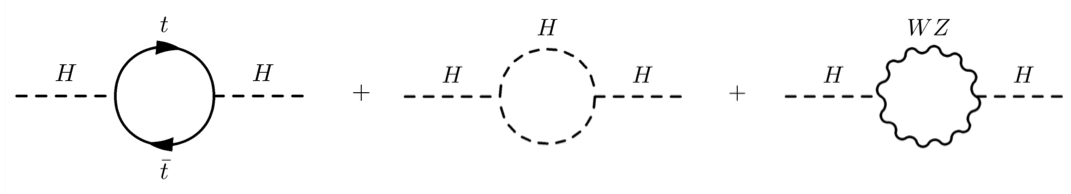
\includegraphics[width=15cm]{SM_chapter_plots/higgsmass}
\caption{Radiative Corrections to the Higgs Mass. \label{figurehiggsmass}}
\end{figure}
\begin{eqnarray}\label{higgsmasseq}
m_{H}^{2} = m_{H,0}^{2} + \dfrac{3 g^{2}}{32 \pi^{2}}\dfrac{\Lambda^{2}}{m_{W}^{2}}\left[ m_{H}^{2} + 2m_{W}^{2} + m_{Z}^{2} - \dfrac{4}{3} m_{t}^{2}  \right] 
\end{eqnarray}
To avoid this, one
has to adjust the Higgs bare mass $m_{H,0}$ to one
part in $10^{17}$. This is quite unnatural, and is what we call the
gauge \textbf{hierarchy problem}.
In order to solve this unnatural fine tunning some theories beyond SM were proposed, for example, Supersymmetry (SUSY), Composite Higgs and Extra Dimensions. We will focus only in the last of these models.

\subsection{Dark Matter}

Dark matter is a hypothetical kind of matter that cannot be seen with telescopes but accounts for most of the matter in the universe. Dark matter neither emits nor absorbs light or any other electromagnetic radiation at any significant level. This means that it has not electric charge and can interact only via gravitational force, or weak force similar to neutrinos.
The existence and properties of dark matter are inferred from many sources,
\paragraph{Velocity curves of spinning galaxies} In 1970 an American astronomer, Vera Rubin, measured the speed of stars in rotating galaxies accurately enough to convince the scientific community. She observed that stars in spinning galaxies were all rotating at roughly the same velocity, no matter their distance to the galactic centre. This is in contradiction with Kepler’s law that describes the rotation of planets around the Sun.  This could only happen if huge amounts of invisible matter filled the entire galaxy and beyond.
\paragraph{Gravitational lensing} We know that light moves in a straight line in free space. In the presence of a massive object such as a star or a galaxy, the space is deformed and light follows the curvature of the distorted space. Light coming from a distant galaxy will bend when passing near a massive clump of dark matter and the galaxy will appear shifted, as if coming from different places.
\paragraph{Cosmic microwave background} Astrophysicists can infer how much dark matter exists by studying the cosmic microwave background. From the amount of radiation associated to each frequency, astrophysicists can calculate the quantity of dark matter contained in the Universe.\\

\indent Experiments at the (LHC) may supply more direct evidence about dark matter. According to many theories, dark matter particles would be light enough to be produced at the LHC. If they were generated at the LHC, they would escape through the detectors leaving no signal. However, they would transport energy and momentum, so one could infer their existence from the amount of energy and momentum "missing" after a collision. Dark matter candidates arise frequently in theories that suggest physics beyond the Standard Model, such as Supersymmetry and Extra Dimensions.

\subsection{Extra Dimensions}

Why is gravity so much weaker than the other fundamental forces?  One possibility is that we don’t feel the full effect of gravity  because part of it spreads to extra dimensions. If extra dimensions exist, they could explain why gravity is weaker than the other forces of nature.

How could we test for extra dimensions? 
Some theorists suggest that a particle called the "graviton" is associated with gravity. If gravitons exist, it should be possible to create them at the LHC, but they would rapidly disappear into extra dimensions. A graviton might escape our detectors, leaving an empty zone that we notice as an imbalance in momentum and energy in the event. We would need to carefully study the properties of the missing object to work out whether it is a graviton escaping to another dimension or something else. This method of searching for missing energy in events is also used to look for dark matter or supersymmetric particles.

	

\subsubsection{Large Extra Dimensions}

The reason why we have not observed the extra dimensions yet is that contrary to the ordinary four space-time dimensions which are very large (or infinite), these hypothetical extra dimensions are finite, that is they are compactified. The  question that one needs to ask is how large could the size of the extra dimensions be without getting into conflict with observations.\\
\indent 
Assuming that there are $n$ extra dimensions, calling the fundamental Planck scale of the theory (in $4+n$ dimension) $M_{*}$, the usual Planck scale (in 4 dimensions) $M_{Pl}$, $r$ the compactification radius of the extra dimension, and using the matching for the gravitational and the gauge coupling, it is found that \cite{Csaki:2004ay}:
\begin{eqnarray}
M_{Pl}^{2} &=& M_{*}^{n+2}V_{(n)}= M_{*}^{n+2}\left(2 \pi r \right)^{n} \sim r^{n}M_{*}^{n+2}\label{planck}\\ 
\dfrac{1}{g_{4}^{2}} &=& V_{(n)}M_{*}^{n} \sim r^{n}M_{*}^{n}
\end{eqnarray}
In the second equation we assume that the gauge field propagates in all dimensions. Considering that the spacetime is flat, and that the $n$ extra dimensions are compact, where $V_{n}$ is the volume of the extra dimensional space and $g_{4}$ is the coupling constant. From these two equations it is obtainned:
\begin{eqnarray}
r \sim \dfrac{1}{M_{Pl}}\:g_{4}^{\frac{n+2}{n}}
\end{eqnarray}
This would imply that in a higher dimensional theory $r \sim 1/M_{Pl}$. In this case there would be no hope of finding these tiny extra dimensions. Now, we will investigate what happen if, instead of the previous assumption, the SM fields were localized in 4 dimensions, and only gravity were to propagate into the extra dimension. 
In that case new phenomena will appear in the gravitational sector when you reach distances as short as the size of the extra dimension. However, it is very hard to test gravity at very short distances. The bound in the size of the extra dimension ($r\leq$ \unit[0.1]{mm}) is given by Cavendish type experiments if only gravity propagates in the extra dimension.\\ 
\indent
For $M_{*}\sim$ \unit[1]{TeV} the model is called "Large Extra Dimensions", proposed by Arkani-Hamed, Dimopoulos and Dvali (ADD) \cite{ArkaniHamed:1998rs}.
From (eqn. \ref{planck}) we find:
\begin{eqnarray}
r \sim 2\times 10^{17}\times 10^{\frac{32}{n}} \text{cm}
\end{eqnarray}
Therefore, if we select $n=1$ , we get that $r\sim 10^{8}$ Km, which is certainly excluded. Taking $n=2$ , one has $r \sim 1$ mm, which is a distance scale already constrained by Cavendish-type experiments.\\
\indent
The fact that gravity propagates in compact extra dimensions leads to the existence of graviton excitations with a mass gap given by $\Delta m \sim 1/R$.
The graviton in this $(4+n)$-dimensional formulation can be equivalently expressed as a set of 3-dimensional Kaluza–Klein (KK) modes  with different graviton masses. The coupling of the KK modes to the SM energy–momentum tensor leads to an effective theory with virtual-graviton exchange at leading order (LO) in perturbation theory. An ultraviolet (UV) cutoff must be introduced to avoid divergences in the summed contributions from all modes.


\subsubsection{Universal Extra Dimensions}

Universal Extra Dimensions \cite{PhysRevD.64.035002} are models in which all of the SM fields live in $4+n$ dimensions with the $n$ extra dimensions taken to be flat and compact. 
In the Minimal Universal Extra Dimensions (MUED) we have five dimensions, namely only one extra dimension. In this model the hierarchy problem is not addressed but have some interesting features as a stable dark matter candidate.
In this case the extra dimension is compactified in a circle of radius $r$. 
The key element is the conservation of momentum in the universal dimensions. In the equivalent four-dimensional theory this implies KK number conservation. For example, in five dimensions (5D), $p_{5}$ the fifth component of the 5D momentum is quantified and given by
\begin{eqnarray}
p_{5} = n/r
\end{eqnarray}
Promoting the full SM to extra dimensions bring some problems, for example the fermions are generically non-chiral (with respect to our four dimensions). This problem is solved by "orbifolding", \ie, compactifying on surfaces with endpoints. In five dimensions, the only choice is $S^{1}/Z_{2}$, which identifies opposite sides of a circle to create a line segment with two endpoints.

\begin{figure}[H]
  \centering
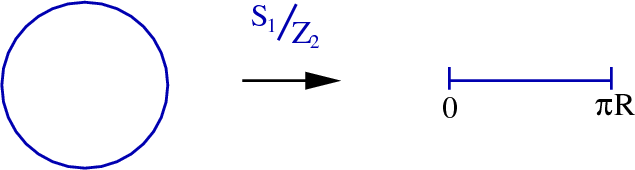
\includegraphics[width=12cm]{SM_chapter_plots/orbifold}
\label{orbifigure}\caption{orbifold}
\end{figure}

As a consequence of the orbifolding, translational invariance along the 5th dimension is broken, which results that the KK-number conservation is broken too, but there is a remnant left: the parity
of the KK modes must be conserved at	 the vertex. In addition, KK-parity conservation means that the lightest state of
the first KK level cannot decay into zero-modes, making it
stable and a candidate for dark matter.
The masses of the KK modes at tree levl are given by:
\begin{eqnarray}
m_{n}^{2} = \dfrac{n^{2}}{r^{2}}+ m_{SM}^{2}
\end{eqnarray}
with $n=0,1,2,\dots$. Note that for $n=0$ (zero mode) we obtain the mass on the SM particles. In general the mass of the SM particles are smaller than the compactification radius of the extra dimension, so the KK modes are practically degenerate. Radiative corrections generate mass splittings, but these are still
small enough for the energy yield to be small in the production and subsequent decay of KK states.

\subsubsection{Warped Extra Dimension}

\paragraph{Randall Sundrum (RS) Models}

Lisa Randall and Raman Sundrum proposed a model where there is only one warped extra dimension which is compactified on the $S^{1}/Z_{2}$ orbifold \cite{Randall:1999ee,Randall:1999vf}. Two 4D branes (the Planck brane and the TeV brane) are separated by the fifth extra dimension with size $r_{c}$ (fig. \ref{RSfigure}). Even though the extra dimension is curved, the brane itself remains static and flat, that is, it preserves 4D Lorentz invariance. This means that the induced metric at every point along the extra dimension has to be the ordinary flat 4D Minkowski metric, and the components of the 5D metric depend only on the fifth coordinate $y$. The ansatz for the most general metric satisfying these properties is given by:
\begin{eqnarray}
ds^{2}= e^{-A(y)} dx^{\mu}dx^{\nu} \eta_{\mu\nu} - dy^{2} 
\end{eqnarray}
Where $\eta_{\mu\nu}=\text{diag}(-1,1,1,1)$ and the amount of curvature (warping) along the extra dimension depends on the function $e^{-A(y)}$, which is therefore called the warp-factor. This
type of geometry is called "non-factorizable" because the metric of the 4D subspace is $y$-dependent.
In the simplest version of the RS model it is assumed that the SM fields live on the so-called TeV brane while gravity lives everywhere. Unlike the ADD case, however, there is a "cosmological" constant in the 5D bulk and both branes have distinct tensions. Solving the 5D Einstein’s equations provides a unique solution for these quantities and also determines that $A(y) = k\left| y \right| $, where k is a dimensionful parameter. A basic assumption of this model is that there are no large mass hierarchies present, so that we expect that $k \sim M_{*}$, the 5D fundamental or Planck scale. In fact, once we solve Einstein’s equations and plug the solutions back into the original action and integrate over $y$ we find that:
\begin{eqnarray}
M_{Pl}^{2} = \dfrac{M_{*}^{3}}{k}\left(1-e^{-2\pi k r_{c}} \right)  
\end{eqnarray}
The warp factor $e^{-\pi k r_{c}}$ will be a very small quantity which implies that $M_{Pl}$, $M_{*}$ and $k$ have essentially comparable magnitudes following from the assumption that no hierarchies exist. If we calculate the Ricci
curvature invariant for this 5D space, we find that it is  constant, $ R_{5} = - 20 k^{2}$ and thus $k$ is a measure of the
constant curvature of this space. A space with constant negative curvature is called an Anti-DeSitter space and so this 5D version is called $AdS_{5}$.
\begin{figure}[H]
  \centering
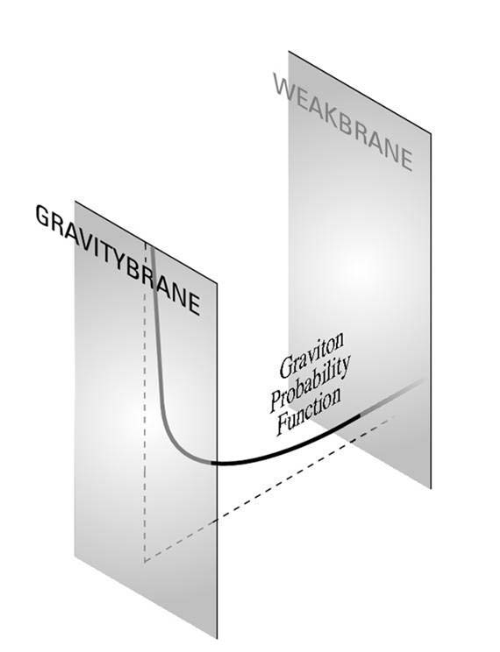
\includegraphics[width=6cm]{SM_chapter_plots/RS}
\caption{Graviton probability function \label{RSfigure}}
\end{figure}

It will be assumed that all dimensionful parameters in the action will have their mass scale set by $M_{*} \sim M_{Pl} \sim k$ so that there is no fine-tuning. However, the warp factor rescales them as one moves about in $y$ so that, in particular, all masses will appear to be of order the
TeV scale on the SM brane. This means that if there is some mass parameter, $m$, in the action which is order $M_{Pl}$, we on TeV brane will measure it to be reduced by the warp factor, i.e., $me^{-\pi k r_{c}}$. Note that if $kr_{c} \sim 11$ (a
small hierarchy) this exponential suppression reduces a mass of order $10^{18}$ GeV to only 1 TeV. Thus the ratio of the weak scale to $M_{Pl}$ is explained through an exponential factor and no large ratios appear anywhere else in the model. It has been shown by Goldberger and Wise \cite{Goldberger:1999un} that values of $kr_{c} \sim 11$ are indeed natural and can be provided by a stable configuration. Hence we have obtained a true solution to the hierarchy problem.
If we consider the action for the Higgs field on the TeV brane:
\begin{eqnarray}
S = \int d^{4}x dy \sqrt{-g} \left(g^{\mu\nu}\partial_{\mu}H^{\dag}\partial_{\nu}H-\left(H^{2}-v_{0}^{2} \right)^{2}\right)\delta\left(y-\pi r_{c} \right)     
\end{eqnarray}
From this we see that the vev that we observe on the SM brane is not $v_{0}$ but
\begin{eqnarray}
v = v_{0} e^{ -\pi k r_{c}}
\end{eqnarray}
which is of order the TeV scale.
Even though gravitons are spin-2, it turns out that their masses
and wave functions are identical to the case of a scalar field in the RS bulk which is far simpler to analyze. If we solve the Klein-Gordon equation, but now in the case of curved space, after a separation of variables via the KK decomposition the solutions are linear combination of $J_{2}$, $Y_{2}$ Bessel functions and the mass of the KK states are given by: 
\begin{eqnarray}
m_{n} = x_{n} k e ^{-\pi r_{c}}
\end{eqnarray}
where $x_{n}$ are roots of $J_{1}(x_{n})=0$. Here $x_{n} = 0, 3.8317, 7.0155, 10.173, \dots$ etc. Since $k e^{-\pi k r_{c}}$ is of the order of a few hundred GeV at most, we see that the KK graviton masses are of similar magnitude with comparable, but unequal, spacing, i.e., the KK gravitons have approximately weak/TeV scale masses. We thus have weak scale graviton KKs with weak scale couplings that should be produced as spin-2 resonances at colliders.

\paragraph{Bulk Graviton Model}

Different models with warped extra dimensions allow the SM fields to propagate in the ED. In these models, as a consequence of the localization of SM particles near the Planck or the TeV brane, decays to diphotons and dileptons are suppressed by a factor proportional to the volume of the extra dimension. This scenario is more compatible with electroweak precision tests and limits on flavor-changing neutral current processes than the original RS1. The different couplings of the graviton to the SM fields result in two distinctive effects: the branching fraction to SM vector-boson pairs can become dominant for certain values of the model parameters, and a very strong enhancement in the longitudinal polarization of the vector bosons is predicted. Because of the aforementioned suppression of photon and fermion couplings, the total production cross section is also smaller with respect to RS1 gravitons: in the Agashe–Davoudiasl–Perez–Soni (ADPS) model \cite{Agashe:2007zd} for $M = 700$ GeV and $\tilde{k}= 0.50$ , it amounts to 0.31 pb in pp collisions at $\sqrt{s} = 7$ TeV, and the branching fraction to longitudinally polarized ZZ bosons is about 12$\%$.



